\documentclass[11pt,a4paper]{article}
\usepackage[margin=19mm]{geometry}
\usepackage{booktabs,longtable,graphicx,amsmath,hyperref}
\hypersetup{hidelinks}
\setlength{\LTpre}{5pt}
\setlength{\LTpost}{9pt}
\begin{document}
\begin{center}
{\Large Supplementary simulation results}\\[4pt]
{\large Task-Specified Path--Speed Preference Control for an Autonomous Single-Track Robot}\\[5pt]
2026-11-02
\end{center}

\section*{Reading the evidence}
This supplement gives the route-level data omitted from the focused article. All scores use the same original world-frame path and destination, a 10~s observation window, and the frozen task contract. ``Goal'' means entry into the original 1~m destination disk; H10 means upright survival throughout. A narrow pass additionally needs a buffered path corridor and 8--10~s original-path return. A wide pass adds an actual mean turn speed of at least 85\% of the request. The 0.5~m circular buffer is an anchor-based vehicle-envelope proxy. Counts by route use two paired prepared states, not independent policy-training seeds.

U170 is one frozen preference-conditioned middle network. Each $\alpha\in\{0,0.25,0.5,0.75,1\}$ is an input to the same weights. H75 is a separate earlier checkpoint. The geometric rule uses no middle-network output; all matched rows share the lower balance stack and 10~Hz causal path reconnection. The new nominal task combinations were declared before execution. Signed pulses, physical-domain extrema and 90$^\circ$ routes were added after earlier outcomes had been inspected and are exploratory. Physical-domain and nominal panels have different prepared states and must be read separately.

\section{Training review}
The U170 continuation record spans updates 53--202. Its sampled training reward changes with the rollout distribution and is not a fixed-task performance curve. The source log records 150 updates, 2376 accepted minibatches, zero physical failures, 119 domain exits and three target-KL-shortened updates (155, 175 and 188). The frozen checkpoint is assessed by the executed task panels below. Figure~\ref{fig:training} shows the saved reward, domain-exit, KL and critic-loss trends.

\begin{figure}[ht]
\centering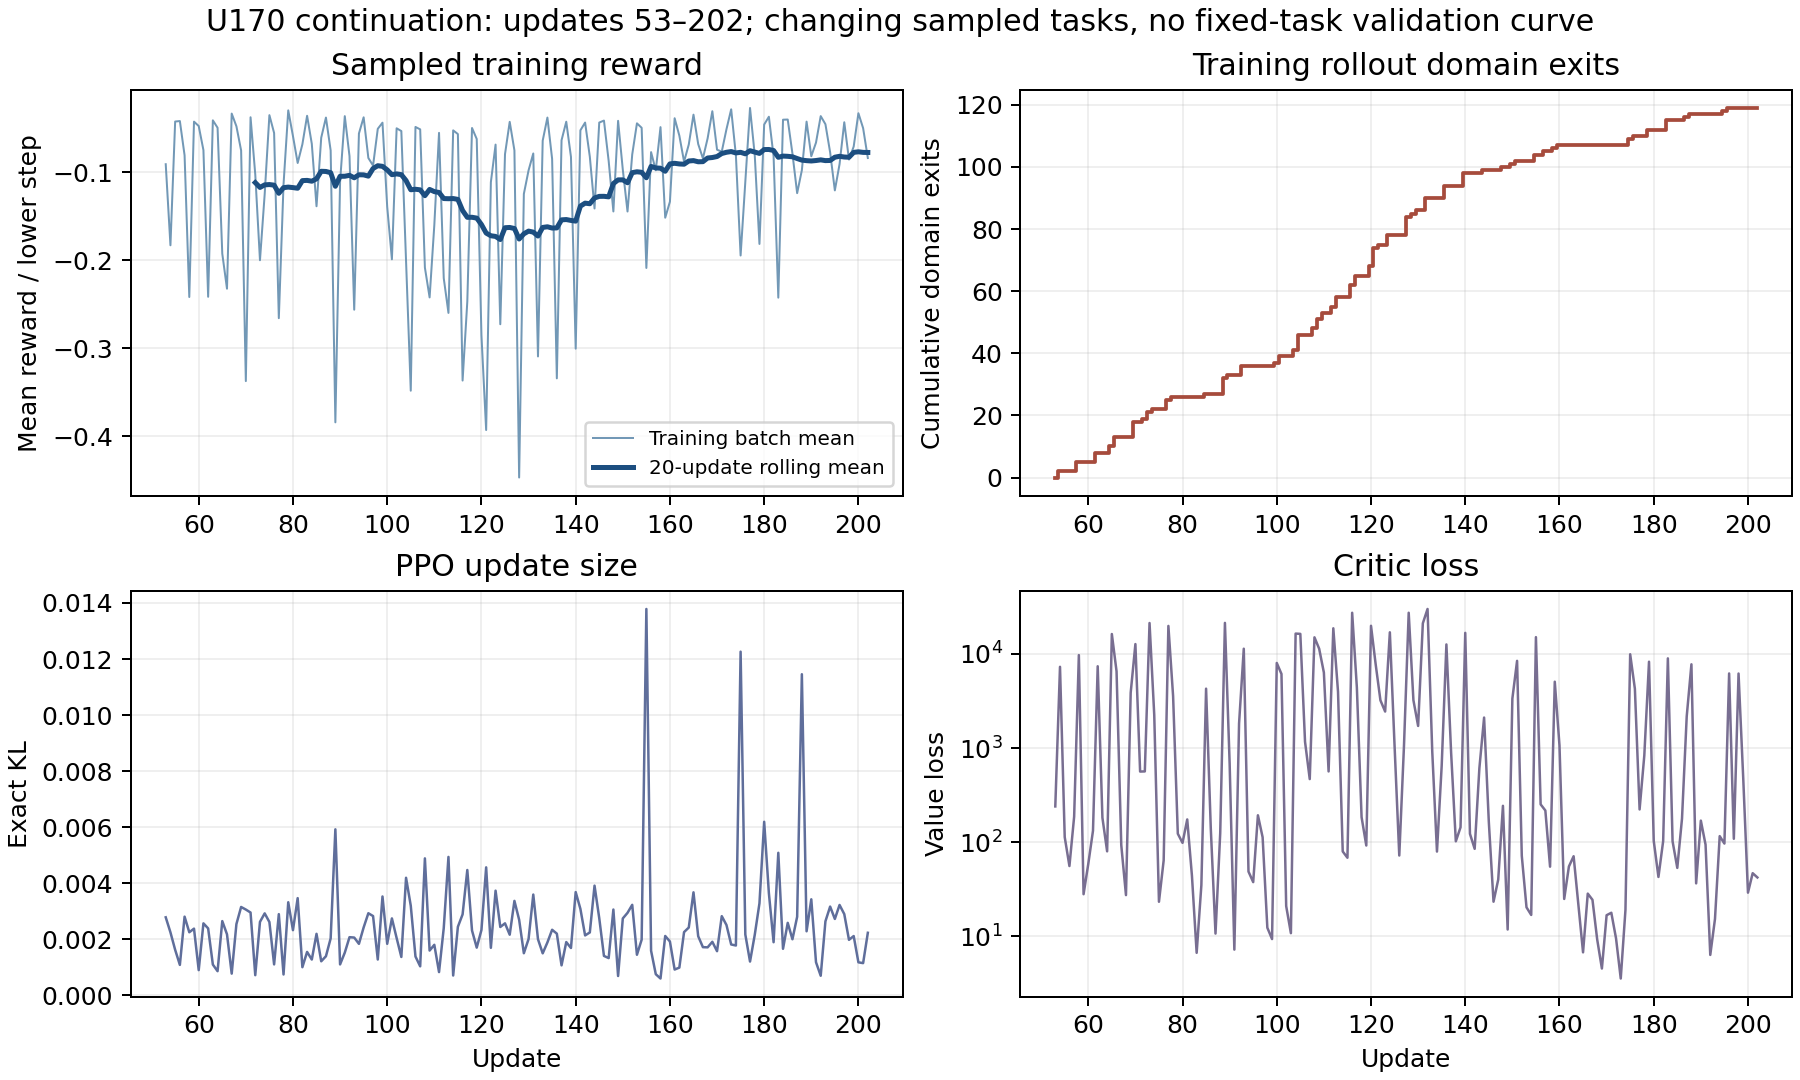
\includegraphics[width=.85\textwidth]{../results/sttw-tolerance-20261101/training_review/training_progress.png}
\caption{Sampled training diagnostics from the archived U170 continuation.}\label{fig:training}
\end{figure}

\begin{longtable}{lrrrrr}
\caption{U170 training windows; reward values are mean per sampled step.}\\
\toprule
Window & Updates & Reward & SD & Domain exits & Exact KL \\
\midrule
\endfirsthead
\toprule
Window & Updates & Reward & SD & Domain exits & Exact KL \\
\midrule
\endhead
Early & 53--92 & -0.1075 & 0.0890 & 33 & 0.0021 \\
Middle & 108--147 & -0.1458 & 0.1154 & 53 & 0.0025 \\
Late & 163--202 & -0.0763 & 0.0457 & 12 & 0.0029 \\
\bottomrule
\end{longtable}

\section{New nominal task combinations}
Four exact low/high single/S route--speed combinations were run from prepared banks 2 and 5. Table~\ref{tab:nominal} reports every route and preference for both H75 and U170. Each row has two physical episodes; all 80 episodes reached the original goal and survived H10. The task completion columns add the path, return and speed tests stated above. Turn speed is the true vehicle-forward speed averaged over the declared turn interval. ``Max cross'' is maximum absolute original-path cross-track error before first goal entry.

\begin{longtable}{llrrrrr}
\caption{Nominal task outcomes by frozen checkpoint, route and preference.\label{tab:nominal}}\\
\toprule
Model & Route & $\alpha$ & Narrow & Wide & Speed & Max cross \\
\midrule
\endfirsthead
\toprule
Model & Route & $\alpha$ & Narrow & Wide & Speed & Max cross \\
\midrule
\endhead
H75 & High S L & 0 & 2/2 & 2/2 & 2.781 & 0.247 \\
H75 & High S L & 0.25 & 1/2 & 2/2 & 2.836 & 0.403 \\
H75 & High S L & 0.5 & 0/2 & 2/2 & 2.903 & 0.530 \\
H75 & High S L & 0.75 & 0/2 & 2/2 & 2.981 & 0.658 \\
H75 & High S L & 1 & 0/2 & 1/2 & 3.050 & 0.906 \\
H75 & High single R & 0 & 2/2 & 2/2 & 2.667 & 0.300 \\
H75 & High single R & 0.25 & 0/2 & 2/2 & 2.732 & 0.521 \\
H75 & High single R & 0.5 & 0/2 & 2/2 & 2.829 & 0.697 \\
H75 & High single R & 0.75 & 0/2 & 2/2 & 2.941 & 0.852 \\
H75 & High single R & 1 & 0/2 & 0/2 & 3.019 & 0.990 \\
H75 & Low S R & 0 & 2/2 & 2/2 & 1.734 & 0.180 \\
H75 & Low S R & 0.25 & 2/2 & 2/2 & 1.774 & 0.185 \\
H75 & Low S R & 0.5 & 2/2 & 2/2 & 1.840 & 0.187 \\
H75 & Low S R & 0.75 & 2/2 & 2/2 & 1.896 & 0.278 \\
H75 & Low S R & 1 & 1/2 & 2/2 & 1.933 & 0.404 \\
H75 & Low single L & 0 & 2/2 & 1/2 & 1.619 & 0.164 \\
H75 & Low single L & 0.25 & 2/2 & 2/2 & 1.671 & 0.158 \\
H75 & Low single L & 0.5 & 2/2 & 2/2 & 1.729 & 0.150 \\
H75 & Low single L & 0.75 & 2/2 & 2/2 & 1.785 & 0.139 \\
H75 & Low single L & 1 & 2/2 & 2/2 & 1.829 & 0.162 \\
U170 & High S L & 0 & 0/2 & 2/2 & 2.694 & 0.449 \\
U170 & High S L & 0.25 & 0/2 & 2/2 & 2.741 & 0.516 \\
U170 & High S L & 0.5 & 0/2 & 2/2 & 2.790 & 0.594 \\
U170 & High S L & 0.75 & 0/2 & 2/2 & 2.830 & 0.660 \\
U170 & High S L & 1 & 0/2 & 2/2 & 2.887 & 0.720 \\
U170 & High single R & 0 & 2/2 & 0/2 & 2.507 & 0.211 \\
U170 & High single R & 0.25 & 2/2 & 0/2 & 2.544 & 0.364 \\
U170 & High single R & 0.5 & 0/2 & 2/2 & 2.602 & 0.557 \\
U170 & High single R & 0.75 & 0/2 & 2/2 & 2.697 & 0.715 \\
U170 & High single R & 1 & 0/2 & 2/2 & 2.807 & 0.850 \\
U170 & Low S R & 0 & 2/2 & 0/2 & 1.616 & 0.216 \\
U170 & Low S R & 0.25 & 2/2 & 0/2 & 1.647 & 0.229 \\
U170 & Low S R & 0.5 & 2/2 & 0/2 & 1.682 & 0.242 \\
U170 & Low S R & 0.75 & 2/2 & 2/2 & 1.719 & 0.256 \\
U170 & Low S R & 1 & 2/2 & 2/2 & 1.762 & 0.278 \\
U170 & Low single L & 0 & 2/2 & 0/2 & 1.558 & 0.215 \\
U170 & Low single L & 0.25 & 2/2 & 0/2 & 1.593 & 0.227 \\
U170 & Low single L & 0.5 & 2/2 & 2/2 & 1.637 & 0.241 \\
U170 & Low single L & 0.75 & 2/2 & 2/2 & 1.691 & 0.259 \\
U170 & Low single L & 1 & 2/2 & 2/2 & 1.744 & 0.280 \\
\bottomrule
\end{longtable}

\section{Signed-force pulse extension}
A world-fixed signed 36~N force was applied at 2.8--2.95~s on the same four routes and banks. Table~\ref{tab:pulse} groups the full 48-case matrix by route, sign and method (two states per row). All 48 remained upright. The positive example in the article is the $+36$~N low S right and high single right subset. Table~\ref{tab:positive} exposes those four matched route--state contexts without aggregating away speed, path deviation, goal entry or the 8--10~s return error. The subset was identified after viewing the full matrix; the negative sign and other routes remain in Table~\ref{tab:pulse}.

\begin{longtable}{lllrrrrr}
\caption{Full signed-pulse matrix grouped over two prepared states.\label{tab:pulse}}\\
\toprule
Route & Force & Method & Goal & Narrow & Wide & Speed & Max cross \\
\midrule
\endfirsthead
\toprule
Route & Force & Method & Goal & Narrow & Wide & Speed & Max cross \\
\midrule
\endhead
High S L & -36 & Rule & 2/2 & 0/2 & 0/2 & 3.038 & 3.057 \\
High S L & -36 & U170 $\alpha=0$ & 2/2 & 0/2 & 0/2 & 2.784 & 2.386 \\
High S L & -36 & U170 $\alpha=1$ & 0/2 & 0/2 & 0/2 & 3.056 & 2.566 \\
High S L & +36 & Rule & 2/2 & 0/2 & 2/2 & 3.034 & 0.664 \\
High S L & +36 & U170 $\alpha=0$ & 2/2 & 0/2 & 2/2 & 2.657 & 0.852 \\
High S L & +36 & U170 $\alpha=1$ & 0/2 & 0/2 & 0/2 & 3.005 & 2.376 \\
High single R & -36 & Rule & 2/2 & 0/2 & 0/2 & 3.022 & 0.541 \\
High single R & -36 & U170 $\alpha=0$ & 2/2 & 0/2 & 0/2 & 2.526 & 0.506 \\
High single R & -36 & U170 $\alpha=1$ & 2/2 & 0/2 & 0/2 & 2.933 & 1.189 \\
High single R & +36 & Rule & 2/2 & 0/2 & 0/2 & 3.004 & 0.465 \\
High single R & +36 & U170 $\alpha=0$ & 2/2 & 0/2 & 0/2 & 2.476 & 0.465 \\
High single R & +36 & U170 $\alpha=1$ & 2/2 & 0/2 & 2/2 & 2.769 & 0.503 \\
Low S R & -36 & Rule & 2/2 & 0/2 & 0/2 & 1.946 & 1.446 \\
Low S R & -36 & U170 $\alpha=0$ & 1/2 & 0/2 & 0/2 & 1.750 & 2.060 \\
Low S R & -36 & U170 $\alpha=1$ & 1/2 & 0/2 & 0/2 & 1.875 & 1.976 \\
Low S R & +36 & Rule & 1/2 & 0/2 & 0/2 & 1.972 & 1.000 \\
Low S R & +36 & U170 $\alpha=0$ & 2/2 & 1/2 & 0/2 & 1.640 & 0.368 \\
Low S R & +36 & U170 $\alpha=1$ & 2/2 & 2/2 & 2/2 & 1.807 & 0.273 \\
Low single L & -36 & Rule & 2/2 & 0/2 & 0/2 & 1.853 & 1.964 \\
Low single L & -36 & U170 $\alpha=0$ & 0/2 & 0/2 & 0/2 & 1.563 & 3.083 \\
Low single L & -36 & U170 $\alpha=1$ & 0/2 & 0/2 & 0/2 & 1.744 & 2.163 \\
Low single L & +36 & Rule & 2/2 & 0/2 & 0/2 & 1.853 & 1.260 \\
Low single L & +36 & U170 $\alpha=0$ & 0/2 & 0/2 & 0/2 & 1.558 & 2.545 \\
Low single L & +36 & U170 $\alpha=1$ & 0/2 & 0/2 & 0/2 & 1.745 & 2.253 \\
\bottomrule
\end{longtable}

\begin{longtable}{lrlrrrrr}
\caption{Individual matched cases in the illustrated $+36$~N positive subset.\label{tab:positive}}\\
\toprule
Route & Bank & Method & Goal & Wide & Speed & Max cross & Return RMS \\
\midrule
\endfirsthead
\toprule
Route & Bank & Method & Goal & Wide & Speed & Max cross & Return RMS \\
\midrule
\endhead
Low S R & 2 & Rule & 0 & 0 & 1.969 & 1.406 & 0.872 \\
Low S R & 2 & U170 $\alpha=0$ & 1 & 0 & 1.638 & 0.476 & 0.140 \\
Low S R & 2 & U170 $\alpha=1$ & 1 & 1 & 1.789 & 0.268 & 0.103 \\
Low S R & 5 & Rule & 1 & 0 & 1.975 & 0.595 & 0.638 \\
Low S R & 5 & U170 $\alpha=0$ & 1 & 0 & 1.642 & 0.261 & 0.114 \\
Low S R & 5 & U170 $\alpha=1$ & 1 & 1 & 1.824 & 0.278 & 0.095 \\
High single R & 2 & Rule & 1 & 0 & 3.009 & 0.466 & 1.199 \\
High single R & 2 & U170 $\alpha=0$ & 1 & 0 & 2.470 & 0.440 & 0.133 \\
High single R & 2 & U170 $\alpha=1$ & 1 & 1 & 2.761 & 0.502 & 0.062 \\
High single R & 5 & Rule & 1 & 0 & 3.000 & 0.464 & 1.276 \\
High single R & 5 & U170 $\alpha=0$ & 1 & 0 & 2.482 & 0.490 & 0.134 \\
High single R & 5 & U170 $\alpha=1$ & 1 & 1 & 2.776 & 0.503 & 0.048 \\
\bottomrule
\end{longtable}

\section{Physical-domain and prepared-state transfer}
The two domain models were selected from an existing four-draw TEST set by the maximum and minimum wheel-friction values. Domain 0 used wheel friction 0.932 and chassis mass scale 0.975; domain 3 used 0.612 and 1.074. Each domain used its own complete prepared banks 0 and 6. Table~\ref{tab:domain} gives every domain/route/method grouping. All 48 physical episodes reached the original destination and survived H10. The new task protocol was applied after earlier outcomes were inspected, so these data show behavior in two sampled domains rather than an untouched generalization estimate.

\begin{longtable}{rllrrrr}
\caption{Task transfer by physical domain, original route and method.\label{tab:domain}}\\
\toprule
Domain & Route & Method & Narrow & Wide & Speed & Max cross \\
\midrule
\endfirsthead
\toprule
Domain & Route & Method & Narrow & Wide & Speed & Max cross \\
\midrule
\endhead
0 & High S L & Rule & 2/2 & 2/2 & 3.054 & 0.112 \\
0 & High S L & U170 $\alpha=0$ & 0/2 & 2/2 & 2.692 & 0.454 \\
0 & High S L & U170 $\alpha=1$ & 0/2 & 2/2 & 2.880 & 0.707 \\
0 & High single R & Rule & 2/2 & 2/2 & 3.012 & 0.108 \\
0 & High single R & U170 $\alpha=0$ & 2/2 & 0/2 & 2.512 & 0.209 \\
0 & High single R & U170 $\alpha=1$ & 0/2 & 2/2 & 2.805 & 0.858 \\
0 & Low S R & Rule & 1/2 & 1/2 & 1.957 & 0.456 \\
0 & Low S R & U170 $\alpha=0$ & 2/2 & 0/2 & 1.614 & 0.217 \\
0 & Low S R & U170 $\alpha=1$ & 2/2 & 2/2 & 1.764 & 0.279 \\
0 & Low single L & Rule & 1/2 & 1/2 & 1.847 & 0.299 \\
0 & Low single L & U170 $\alpha=0$ & 2/2 & 0/2 & 1.559 & 0.216 \\
0 & Low single L & U170 $\alpha=1$ & 2/2 & 2/2 & 1.738 & 0.278 \\
3 & High S L & Rule & 2/2 & 2/2 & 3.044 & 0.104 \\
3 & High S L & U170 $\alpha=0$ & 0/2 & 2/2 & 2.680 & 0.445 \\
3 & High S L & U170 $\alpha=1$ & 0/2 & 2/2 & 2.870 & 0.705 \\
3 & High single R & Rule & 2/2 & 2/2 & 3.004 & 0.107 \\
3 & High single R & U170 $\alpha=0$ & 2/2 & 0/2 & 2.490 & 0.229 \\
3 & High single R & U170 $\alpha=1$ & 0/2 & 2/2 & 2.780 & 0.837 \\
3 & Low S R & Rule & 2/2 & 2/2 & 1.955 & 0.168 \\
3 & Low S R & U170 $\alpha=0$ & 2/2 & 0/2 & 1.639 & 0.225 \\
3 & Low S R & U170 $\alpha=1$ & 2/2 & 2/2 & 1.806 & 0.276 \\
3 & Low single L & Rule & 1/2 & 1/2 & 1.823 & 0.648 \\
3 & Low single L & U170 $\alpha=0$ & 2/2 & 1/2 & 1.647 & 0.204 \\
3 & Low single L & U170 $\alpha=1$ & 2/2 & 2/2 & 1.879 & 0.278 \\
\bottomrule
\end{longtable}

\section{Smooth 90-degree turn experiment}
The added finite-radius original routes change heading by exactly $\pm90^\circ$ at the end of each turn; the source NPZ paths were independently checked. Low-speed requests use 2.0~m/s and radius 1.6~m; high-speed requests use 3.05~m/s and radius 3.0~m, each in left and right directions. Every method used the same two prepared states, original destination and task thresholds. All 48 episodes entered the original goal and survived H10. Table~\ref{tab:angle} gives the complete route/preference grouping. The rule completed both task scores in 8/8 contexts; U170 exhibits a consistent preference response while not exceeding that rule on these turns. Figure~\ref{fig:right} shows the right-turn trajectories omitted from the main article's preselected left-turn figure.

\begin{longtable}{llrrrr}
\caption{All smooth 90$^\circ$ route/preference groupings.\label{tab:angle}}\\
\toprule
Route & Method & Narrow & Wide & Speed & Max cross \\
\midrule
\endfirsthead
\toprule
Route & Method & Narrow & Wide & Speed & Max cross \\
\midrule
\endhead
High 90 L & Rule & 2/2 & 2/2 & 2.996 & 0.113 \\
High 90 L & U170 $\alpha=0$ & 0/2 & 2/2 & 2.758 & 0.622 \\
High 90 L & U170 $\alpha=0.25$ & 0/2 & 2/2 & 2.823 & 0.701 \\
High 90 L & U170 $\alpha=0.5$ & 0/2 & 2/2 & 2.883 & 0.769 \\
High 90 L & U170 $\alpha=0.75$ & 0/2 & 2/2 & 2.935 & 0.827 \\
High 90 L & U170 $\alpha=1$ & 0/2 & 2/2 & 2.973 & 0.881 \\
High 90 R & Rule & 2/2 & 2/2 & 3.010 & 0.112 \\
High 90 R & U170 $\alpha=0$ & 2/2 & 0/2 & 2.509 & 0.214 \\
High 90 R & U170 $\alpha=0.25$ & 2/2 & 0/2 & 2.537 & 0.340 \\
High 90 R & U170 $\alpha=0.5$ & 0/2 & 1/2 & 2.592 & 0.523 \\
High 90 R & U170 $\alpha=0.75$ & 0/2 & 2/2 & 2.683 & 0.679 \\
High 90 R & U170 $\alpha=1$ & 0/2 & 2/2 & 2.793 & 0.810 \\
Low 90 L & Rule & 2/2 & 2/2 & 1.953 & 0.150 \\
Low 90 L & U170 $\alpha=0$ & 2/2 & 0/2 & 1.633 & 0.273 \\
Low 90 L & U170 $\alpha=0.25$ & 2/2 & 0/2 & 1.686 & 0.298 \\
Low 90 L & U170 $\alpha=0.5$ & 2/2 & 2/2 & 1.750 & 0.330 \\
Low 90 L & U170 $\alpha=0.75$ & 2/2 & 2/2 & 1.811 & 0.372 \\
Low 90 L & U170 $\alpha=1$ & 0/2 & 2/2 & 1.867 & 0.431 \\
Low 90 R & Rule & 2/2 & 2/2 & 1.968 & 0.120 \\
Low 90 R & U170 $\alpha=0$ & 2/2 & 0/2 & 1.588 & 0.192 \\
Low 90 R & U170 $\alpha=0.25$ & 2/2 & 0/2 & 1.608 & 0.187 \\
Low 90 R & U170 $\alpha=0.5$ & 2/2 & 0/2 & 1.635 & 0.187 \\
Low 90 R & U170 $\alpha=0.75$ & 2/2 & 0/2 & 1.678 & 0.228 \\
Low 90 R & U170 $\alpha=1$ & 2/2 & 2/2 & 1.750 & 0.285 \\
\bottomrule
\end{longtable}

\begin{figure}[ht]
\centering
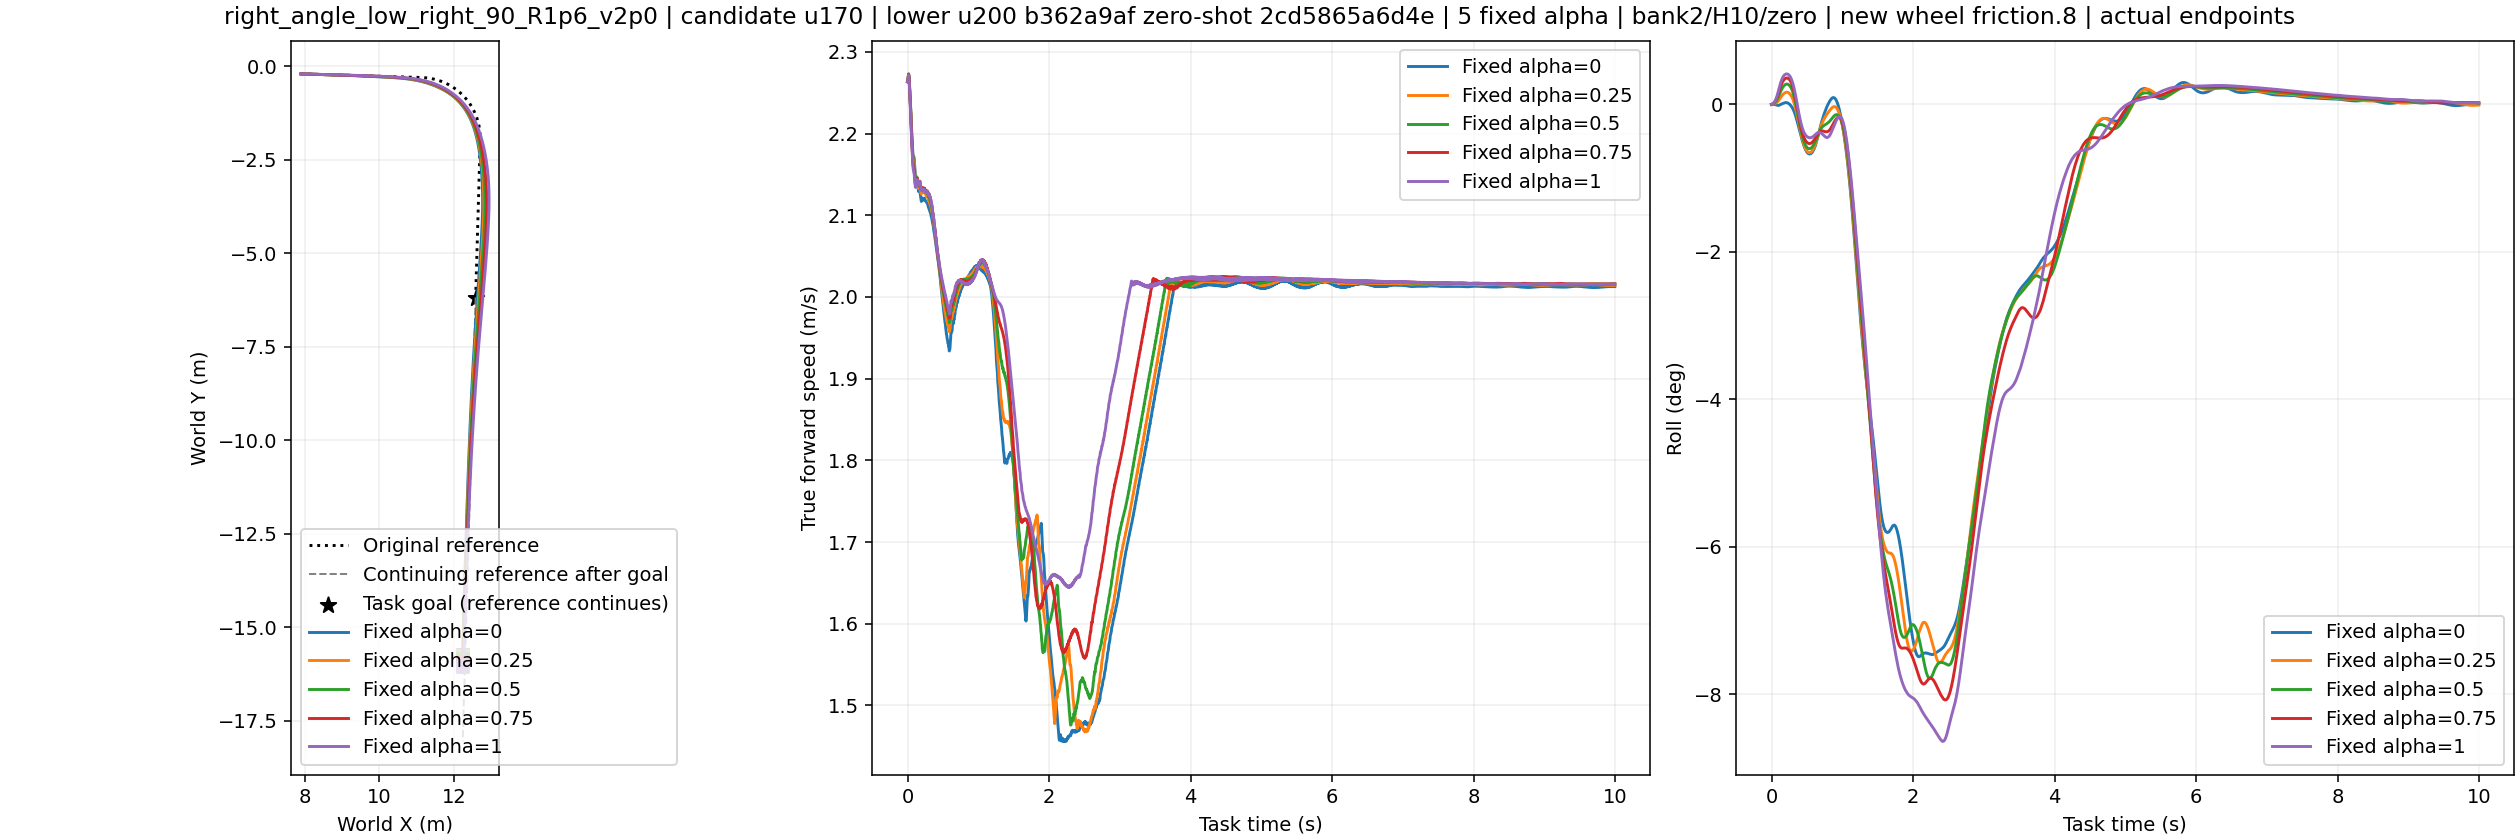
\includegraphics[width=.98\textwidth]{../results/sttw-tolerance-20261101/task_right_angle/xy/u170/bank2_right_angle_low_right_90_R1p6_v2p0_zero_fixed_candidate_xy.png}
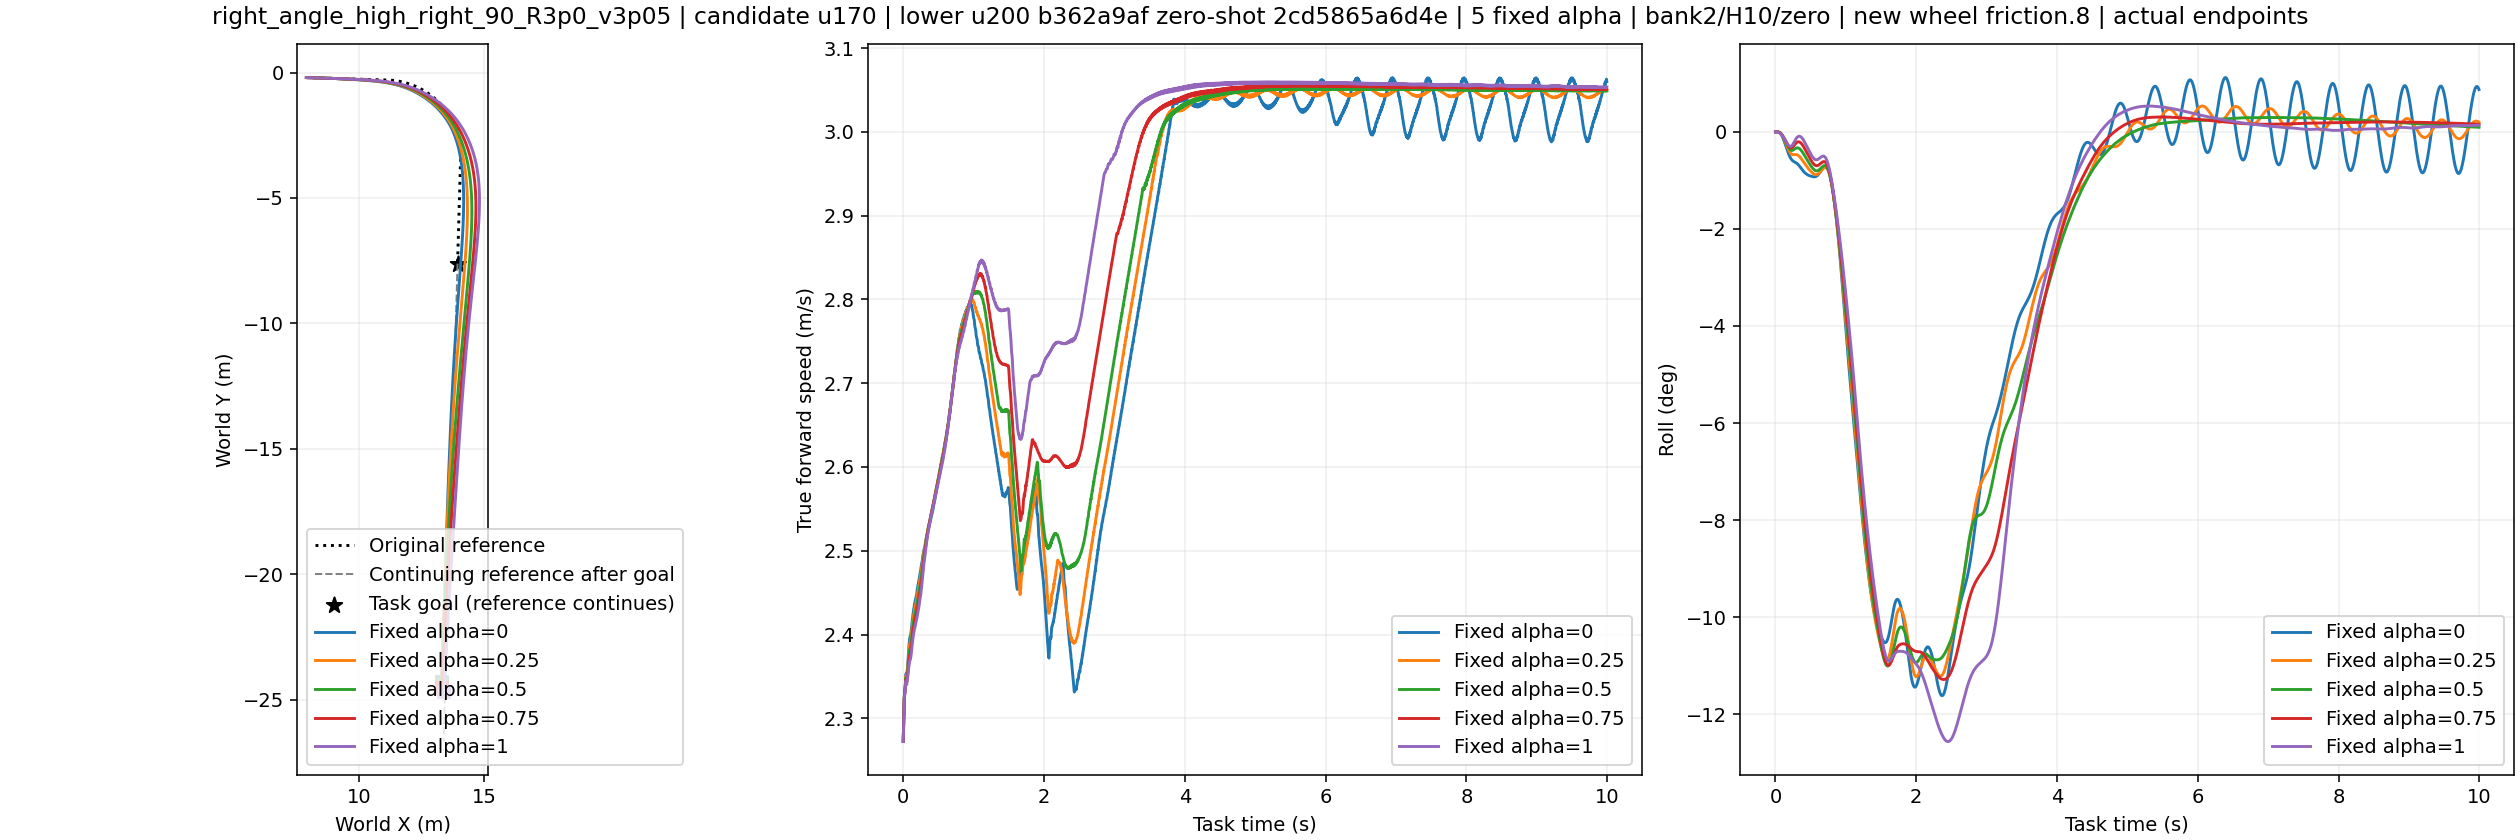
\includegraphics[width=.98\textwidth]{../results/sttw-tolerance-20261101/task_right_angle/xy/u170/bank2_right_angle_high_right_90_R3p0_v3p05_zero_fixed_candidate_xy.png}
\caption{Right 90$^\circ$ turns at low and high requested speed, prepared bank 2: all five U170 preferences, original path, actual speed and roll. The corresponding rule and bank-5 trajectories are in the full result index.}\label{fig:right}
\end{figure}

\begin{figure}[ht]
\centering
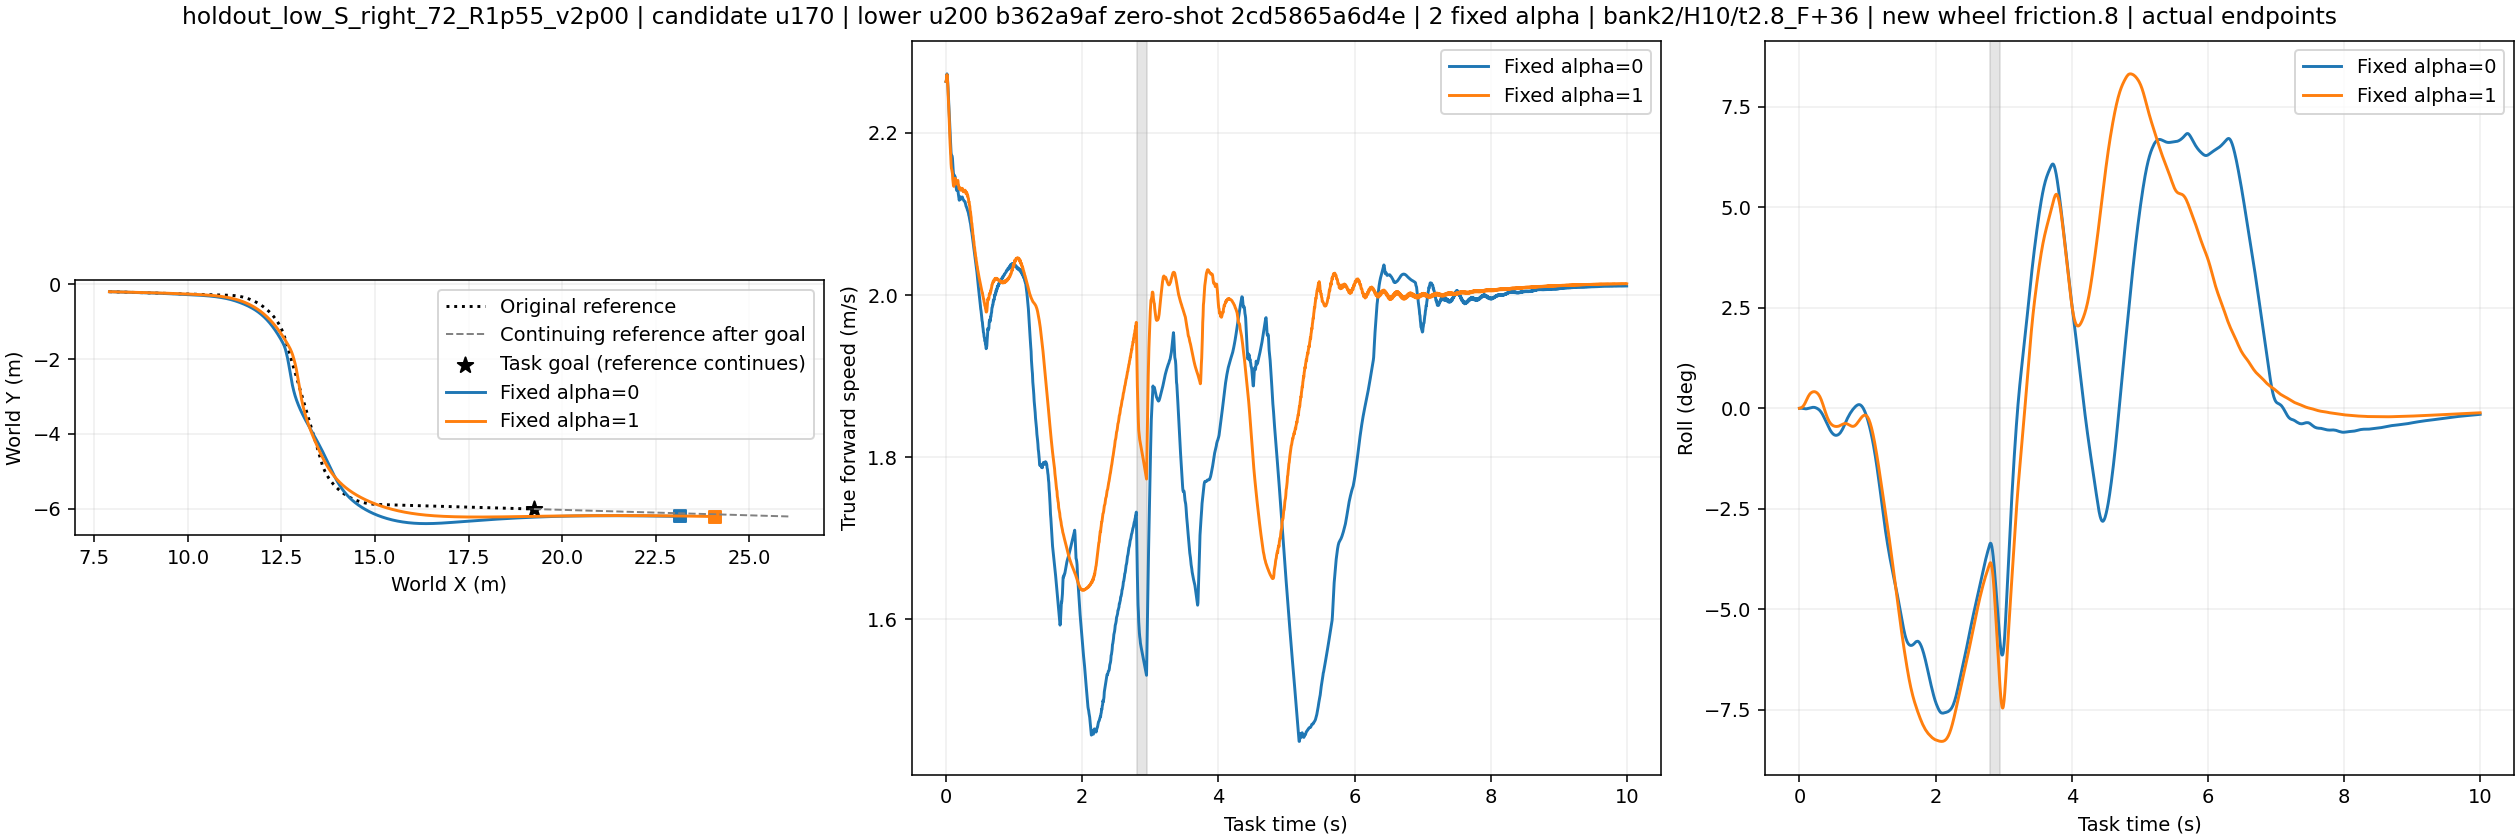
\includegraphics[width=.98\textwidth]{../results/sttw-tolerance-20261101/task_preference_disturbance/xy/u170/bank2_holdout_low_S_right_72_R1p55_v2p00_t2.8_F+36_fixed_candidate_xy.png}
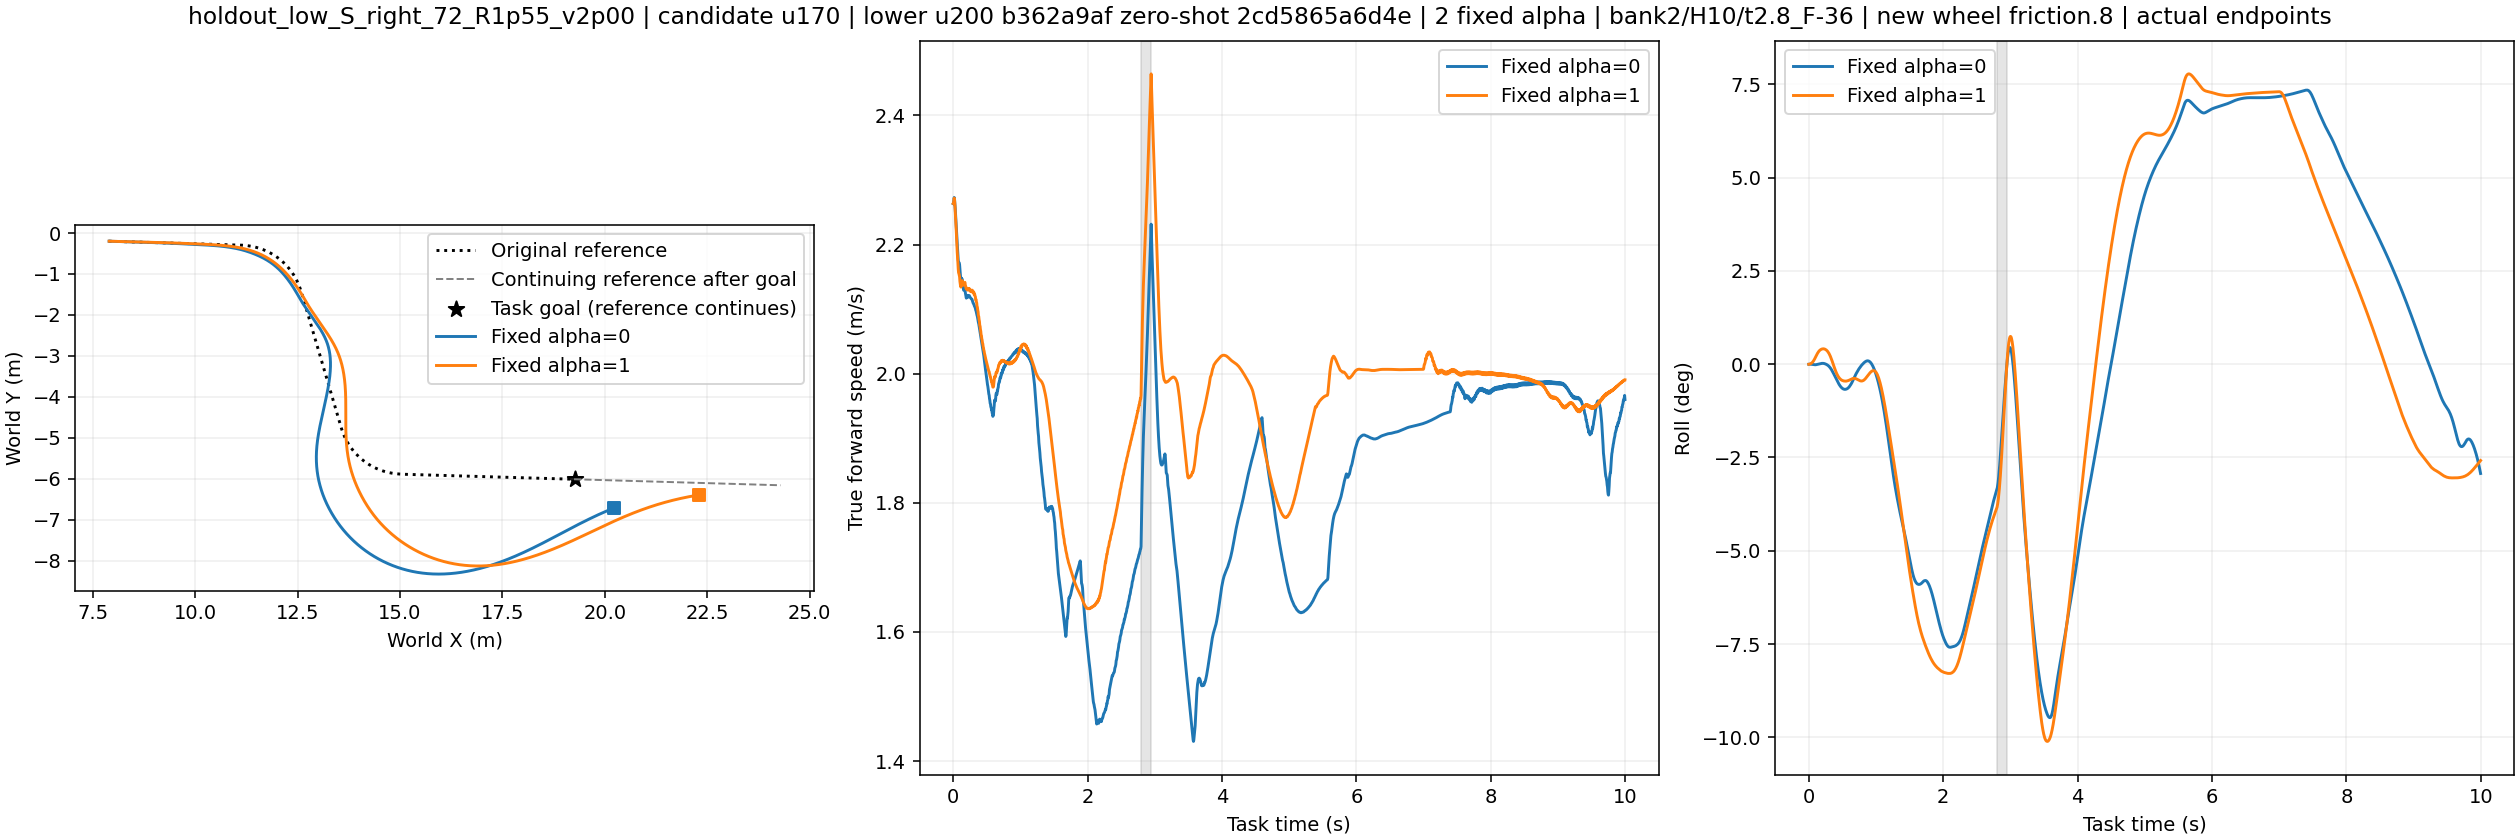
\includegraphics[width=.98\textwidth]{../results/sttw-tolerance-20261101/task_preference_disturbance/xy/u170/bank2_holdout_low_S_right_72_R1p55_v2p00_t2.8_F-36_fixed_candidate_xy.png}
\caption{Same low-speed S right route and prepared bank 2 under the two signed force pulses. The article's positive example uses the upper $+36$~N case; the lower $-36$~N case is retained for direction-specific comparison.}\label{fig:pulsesign}
\end{figure}

\section*{Complete case and raw-trajectory access}
The machine-readable companions retain every individual outcome, including non-arrivals and task failures: \href{../results/sttw-tolerance-20261101/task_preference_holdout/holdout_comparison.json}{nominal cases}, \href{../results/sttw-tolerance-20261101/task_preference_disturbance/comparison.json}{signed pulses}, \href{../results/sttw-tolerance-20261101/task_preference_physical_domain/comparison.json}{physical domains}, and \href{../results/sttw-tolerance-20261101/task_right_angle/comparison.json}{90-degree turns}. Their adjacent Markdown indices link all original/actual XY images and archived raw NPZ trajectories. The current paper package has no new policy training and no hardware results.
\end{document}
